\section{\ref{PS:Q:Availability}}

\textit{Can we create a solution where removing one or more nodes from the system at runtime does not cause system failure?}\newline\newline

\noindent To answer whether or not a fully decentralized current Siemens system can handle removing one or more nodes at runtime, the discussion section of this experiment also contains a discussion with regards to the components analyzed in \cref{cha:stateOfTheArt}: State of the Art.

\subsection{Experiments}
The \ref{PS:Q:Availability} problem address if the proposed decentralized solution is able to continue its functions even though nodes are removed from the system at runtime.
The proposed decentralized solution should be able to continue maintaining the global setpoint of the wind farm even if some turbines become unavailable, assuming that the needed production capacity is present in the park.

The below experiment is repeated with $N = 1, 5, 10, 15$ failing turbines of 30 running turbines.

The experiment has the following procedure:
\begin{enumerate}
	\item Start the system with 30 turbines.
	\item Make sure the system is stable.
	\item Kill N nodes.
\end{enumerate}

Did the system adjust the setpoints for all turbines to maintain the global setpoint?

\subsection{Results}
\label{sec:res:availability}
The plots in \cref{fig:exp:availability_kill15,fig:exp:availability_kill10,fig:exp:availability_kill5,fig:exp:availability_kill1} show how the decentralized solution reacts when killing 1, 5, 10 and 15 turbines. The figures are Matlab screen shots from the graphical interface made with DDS Blockset for Simulink (described in section \cref{sec:graphicalInterface}). The x-axis show Time in seconds and the y-axis show kW production.  The global setpoint is set to 20000~kW for the experiment where 1 turbine is removed (\cref{fig:exp:availability_kill1}). The global setpoint value for this expertiment has been set this high to provide a better visual representation for the case where 1 turbine is crashed (a change of $globalSetpoint/nTurbines=2000kW/30=66,6kW$ is harder to see on \cref{fig:exp:availability_kill1} than change of $20000kW/30=666,6kW$). 

For the remainder of the cases (meaning where 5, 10 and 15 turbines are crashed), the global setpoint is set to 2000~kW.

The turbines are all running with a cycle time of 20 ms throughout this experiment.

\Cref{fig:exp:availability_kill1} shows an increase of production pr. turbine by approximately 20 kW pr. remaining turbines, after a single turbine is crashed. A global setpoint of 20000kW was set for this test.

\begin{figure} [!h]
	\centering
	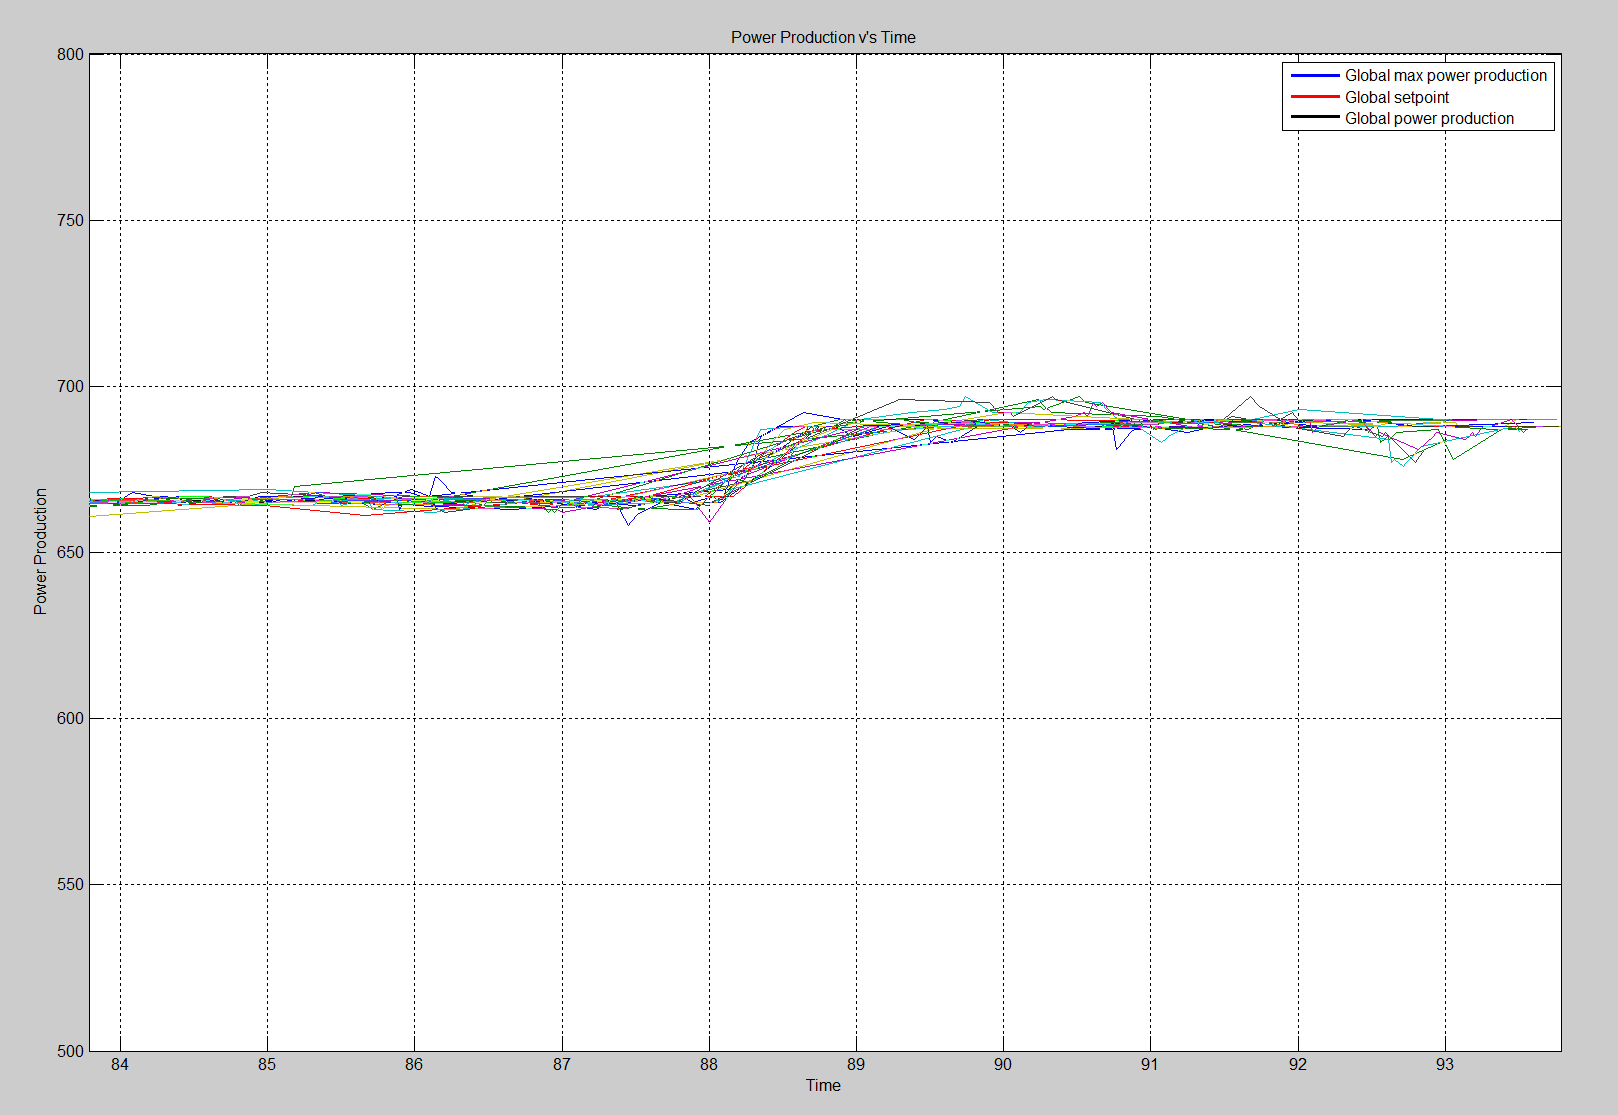
\includegraphics[width=\resultsFigureWidthScale\textwidth]{figures/Results/availabilitytest30-29_setpoint_20000.PNG}
	\caption{Availability test kill 1 out of 30 turbines}
	\label{fig:exp:availability_kill1}
\end{figure}

\Cref{fig:exp:availability_kill5} shows an increase of production pr. turbine by approximately 15 kW pr. remaining turbines, after 5 turbines are crashed. A global setpoint of of 2000kW was set for this test.

\begin{figure} [!h]
	\centering
	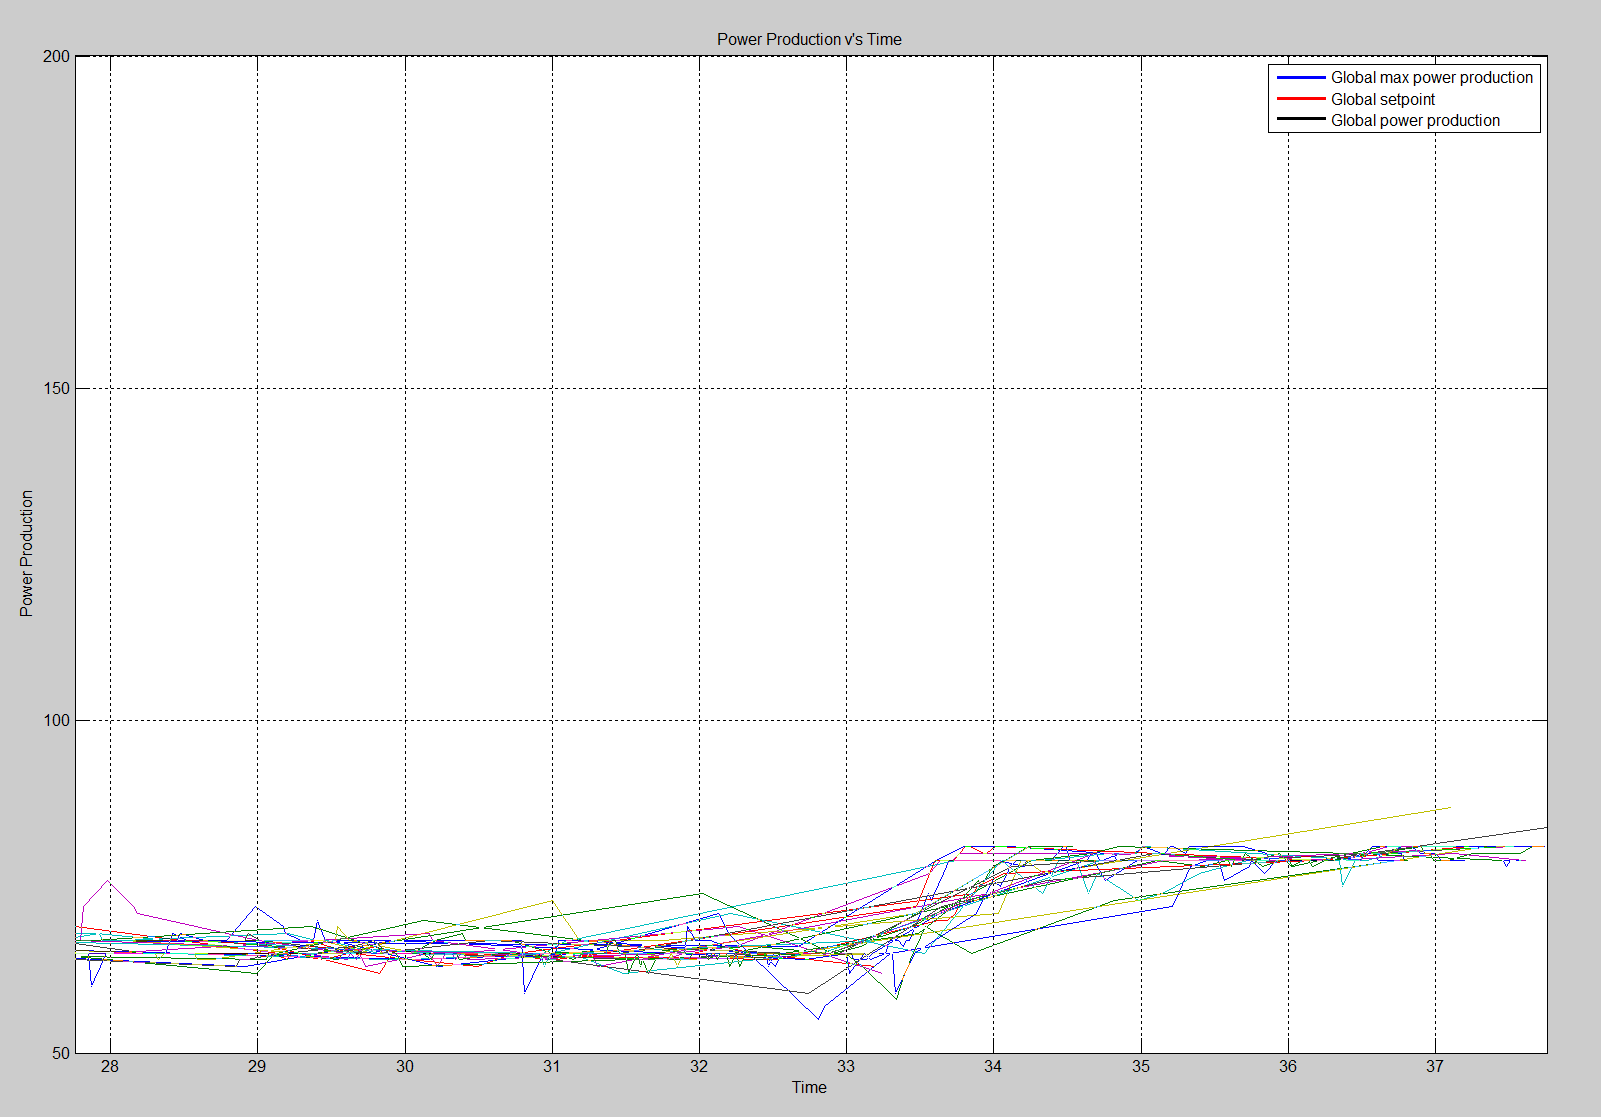
\includegraphics[width=\resultsFigureWidthScale\textwidth]{figures/Results/availabilitytest30-25_setpoint_2000.PNG}
	\caption{Availability test kill 5 out of 30 turbines}
	\label{fig:exp:availability_kill5}
\end{figure}

\Cref{fig:exp:availability_kill10} shows an increase of production pr. turbine by approximately 30 kW pr. remaining turbines, after 10 turbines are crashed. A global setpoint of of 2000kW was set for this test.

\begin{figure}[!h]
	\centering
	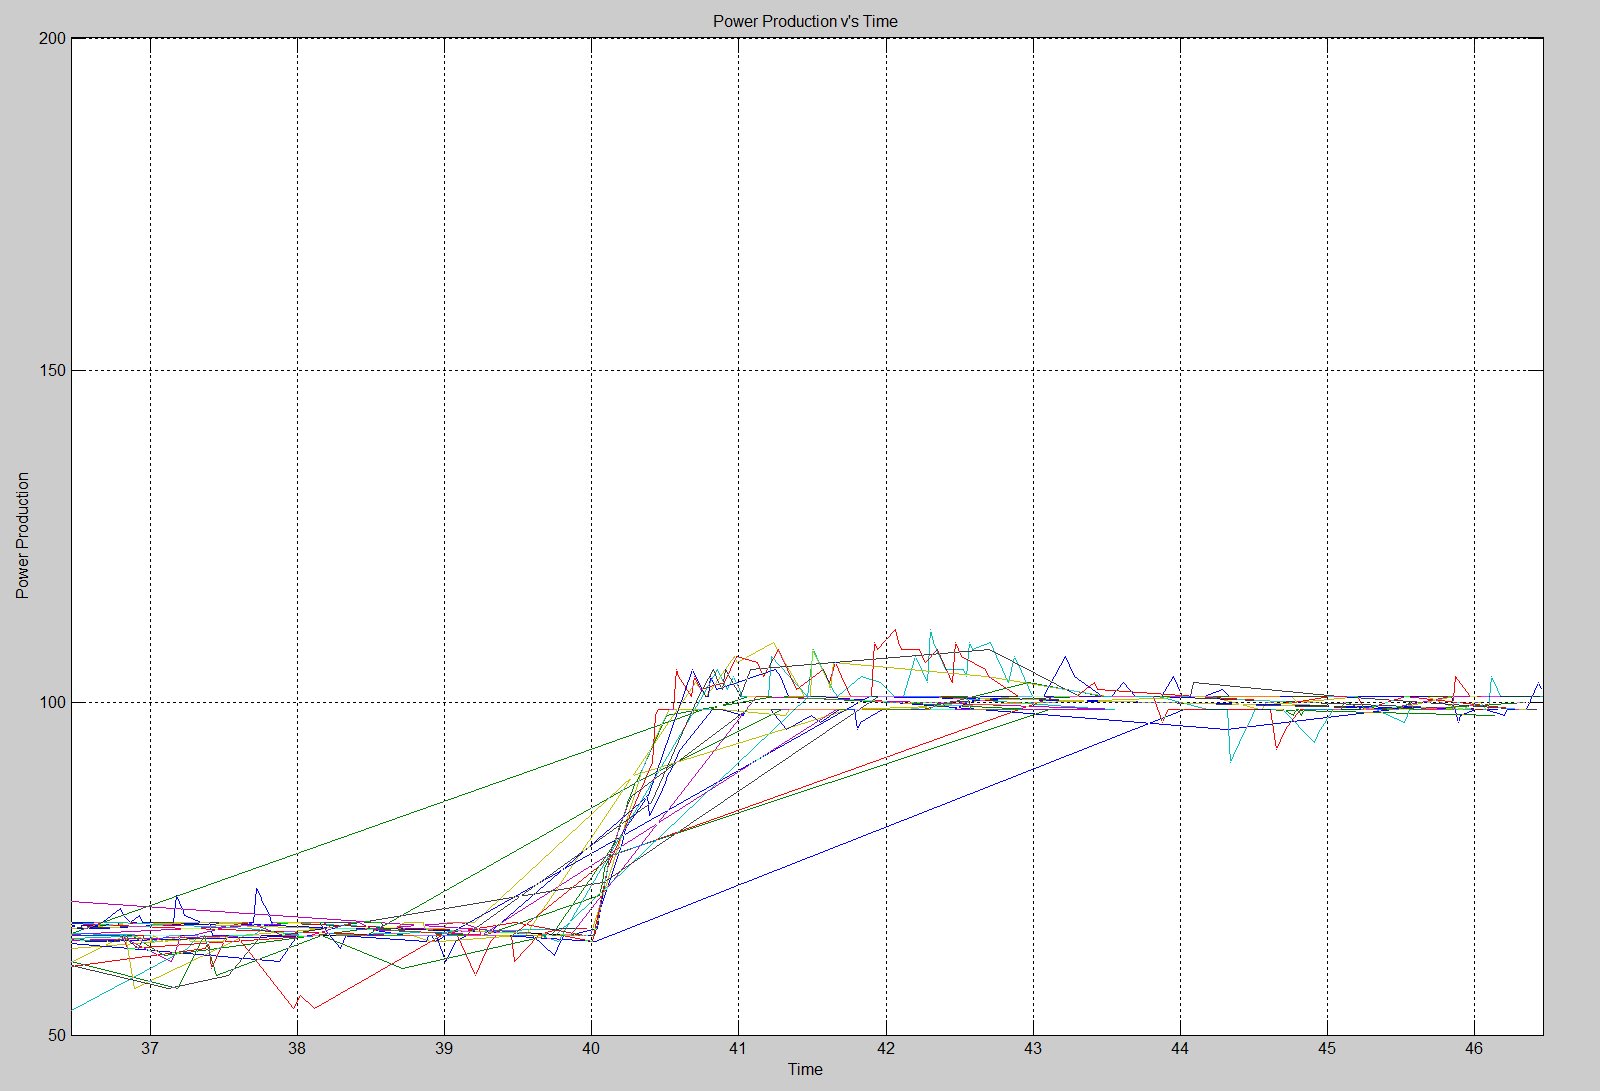
\includegraphics[width=\resultsFigureWidthScale\textwidth]{figures/Results/availabilitytest30-20_setpoint_2000.PNG}
	\caption{Availability test kill 10 out of 30 turbines}
	\label{fig:exp:availability_kill10}
\end{figure}

\Cref{fig:exp:availability_kill15} shows an increase of production pr. turbine by approximately 60 kW pr. remaining turbines, after 15 turbines are crashed. A global setpoint of of 2000kW was set for this test.

\begin{figure}[!h]
	\centering
	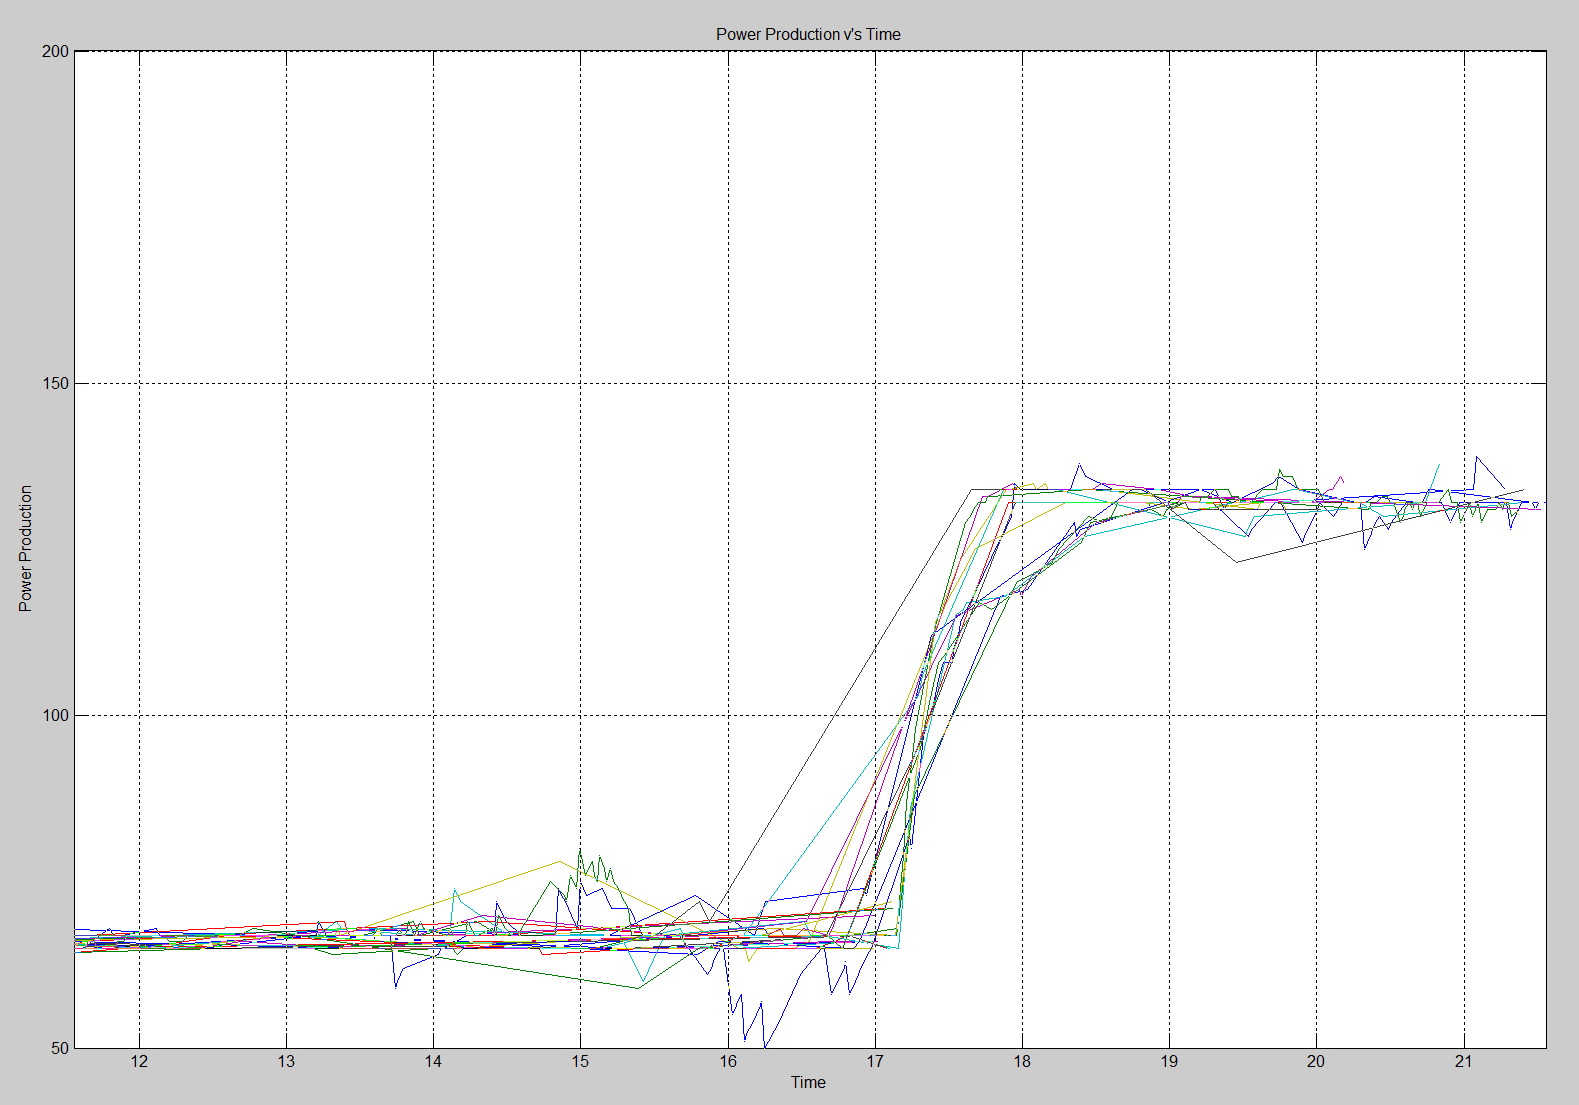
\includegraphics[width=\resultsFigureWidthScale\textwidth]{figures/Results/availabilitytest30-15_setpoint_2000.PNG}
	\caption{Availability test kill 15 out of 30 turbines}
	\label{fig:exp:availability_kill15}
\end{figure}

\FloatBarrier
\subsection{Discussion}
One of the main challenges of decentralized systems is to continue operation in the face of communication failure or node loss. As presented in figures \ref{fig:exp:availability_kill1} to \ref{fig:exp:availability_kill15} the decentralized solution can handle the loss of turbines. A turbine is considered offline if it does not publish any new data to any other turbines within a 150 ms timespan, defined by the Lifespan QoS parameter of the DataWriter described in \cref{sec:decen:ddsconf}.
This upper limit of 150 ms is chosen because 150 ms is the upper limit of the regulation cycle time in the current Simens system.
After turbines has been detected as crashed the remaining turbines in the wind farm will share the load of the missing turbines, to keep the global power production of the park as close to the global setpoint as possible.

Let k = the number of turbines crashed, p = production of the crashed turbine, and n = number of remaining turbines. The expected increase of production pr. turbine when one or more turbines are crashed, is denoted as (by regulation algorithm definition explained in \cref{sec:calculateSetpoints}): $$Production~increase~per~turbine = \frac{\sum\limits_{i=1}^k(p)}{n}$$

Thus the expected production increase for the case where a single turbine is crashed (\cref{fig:exp:availability_kill1}) is: $$\frac{\sum\limits_{i=1}^1(666,6kW)}{29}\approx23kW$$

Hence for the rest of the cases (note that the global setpoint for these cases are 2000kW, thus the production of each turbine is 66,6 kW as apposed to 666,6 kW for the case where one turbine was crashed):
\newline\newline
\noindent5 turbines crashed (\cref{fig:exp:availability_kill5}) $$\frac{\sum\limits_{i=1}^5(66,6kW)}{25}\approx13kW$$

\noindent10 turbines crashed (\cref{fig:exp:availability_kill10}) $$\frac{\sum\limits_{i=1}^{10}(66,6kW)}{20}\approx33kW$$

\noindent15 turbines crashed (\cref{fig:exp:availability_kill15}) $$\frac{\sum\limits_{i=1}^{15}(66,6kW)}{15}\approx67kW$$

These expected values matches the increased productions shown in figures \ref{fig:exp:availability_kill5} to \ref{fig:exp:availability_kill15}. The glitches of the figures are caused by the simulated turbine data and is therefore accepted for the purpose of this experiment. Thus we conclude that the remaining turbines will share the extra load between themselves and continue power production, when a turbines crashed, as expected, which means removing one or multiple turbines from the system does not impede the regulation of the wind farm. 

%The time it takes the decentralized solution to detect a turbine loss and recover power production is dependent on the following parameters:
%
%\begin{itemize}
%	\item Time of turbine loss detection, which is defined by the History QoS to 150 ms, $I$.
%	\item Time between regulation cycles, in the test cases presented in \cref{sec:res:availability} the time is set to 20 ms, $S$.
%	\item Time of calulation of a new setpoint, $C$.
%	\item Time for the turbine to regulate power production according to the new setpoint. In the turbines this process is simulated with a simple regulation that may take several regulation cycles to complete $R$.
%\end{itemize}
%
%Thus the time for recovery of the power production when a turbine failure occurs can be calculated as $T = I + S + C + R$ which translates to $150 ms + 20 ms + C + R = 170 + C + R ms$. This time can be reduced by lowering the time it takes to detect a turbine is offline which increases the likelihood of detecting a delayed turbine as offline, or by lowering the time between regulation cycles which increases the likelihood of cache reads.

The time it takes for the turbines to regulate according to crashed turbines are of course also an important factor. However since we are using an arbitrary regulation algorithm and turbine simulations, we cannot conclude anything with regards to this subject.

% The only thing we can conclude is that the turbines regulate according to multiple crashed turbines relatively fast, meaning that the time it takes for the turbines to regulate according to one or more crashes happens within an acceptable timeframe of 1 to 4 seconds. 

When it comes to availability for the a potential decentralized Siemens Wind Power wind farm, handling the communication for the regulation algorithm run by the Park Pilot is only a small part of the picture. The Wind Power Supervisor handles external communication for the current Siemens system. Thus to completely decentralize a Siemens Wind Power wind farm, a component to handle external communication is needed. To ensure that the wind farm is available to the outside world, in the face of turbine failures, sets special requirements to the component chosen to handle external communication. A component capable of handling this specific problem has been described in \cref{cha:resourceManagement}.

We also need to address the problem of data loss when a turbine is unresponsive. A turbine has several control and measurement points which are continually logged to a local data store. Should a turbine break down, the local data may be destroyed with the turbine. This again sets special requirements to the component handling data storage. In \cref{sec:databaseStorage} the requirements to the data storage component is described and MongoDB was presented as the best choice to solve the availability problem of data storage. MongoDB is capable of automatic replication of data between turbines, such that data is still available should a turbine failure occur. As well as replication MongoDB provides automatic sharding of a database, which enables global data to be stored across a number of nodes, such that no single node contains all global data. This is needed to prevent single point of failures. Furthermore MongoDB supports aggregation of data across turbines to calculate aggregated values as for instance the global production of the wind farm.

Making the decentralized solution robust and able to handle the loss of turbines with regards to internal communication, regulation of power production, external communication and data storage increases the overall availability of the wind farm. 

\clearpage